% !TeX root = RJwrapper.tex
\title{Residuals and Diagnostics for Ordinal Regression Models: An Introduction to the sure package}
\author{by Brandon Greenwell, Andrew McCarthy, Bradley Boehmke and Dungang Liu}

\maketitle

\abstract{
Residual diagnostics is an important topic in the classroom, but it is less often used in practice. Part of the reason for this is that more complex models, like cumulative link models and logistic regression, do not produce standard residuals that are easily interpreted as those in ordinary linear regression. In this paper, we introduce the concept of surrogate residuals and demonstrate there use through the R package \pkg{sure}.
}


%%%%%%%%%%%%%%%%%%%%%%%%%%%%%%%%%%%%%%%%%%%%%%%%%%%%%%%%%%%%%%%%%%%%%%%%%%%%%%%%
\section{Introduction}
%%%%%%%%%%%%%%%%%%%%%%%%%%%%%%%%%%%%%%%%%%%%%%%%%%%%%%%%%%%%%%%%%%%%%%%%%%%%%%%%

Categorical outcomes are encountered frequently in practice across different fields. For example, in medical studies, the outcome of interest is often binary (e.g., presence or absence of a particular disease after applying a treatment). It is also not uncommon for a categorical outcome to have a natural ordering. For instance, in an opinion poll, the response may be satisfaction such as low, medium, and high. In this case, the response is ordered: low $<$ medium $<$ high.

% Logistic and probit regression are popular choices for modelling a binary outcome. The surrogate approach to constructing residuals actually applies to a wide class of general models of the form 
% \begin{equation*}
%   \mathcal{Y} \sim F_a\left(y; \boldsymbol{X}, \boldsymbol{\beta}\right)
% \end{equation*}
% where $F_a\left(\cdot\right)$ is a discrete cumulative distribution function. This includes binary regression as a special case. For example, the probit model has
% \begin{equation*}
%   \mathcal{Y} \sim bernoulli\left[\Phi\left(\boldsymbol{x}^\top\boldsymbol{\beta}\right)\right],
% \end{equation*}
% where $\Phi\left(\cdot\right)$ is the cumulative distribution function for the standard normal distribution.

The \dfn{cumulative link} model is a natural choice for modelling an ordinal outcome. Consider an ordinal categorical outcome $\mathcal{Y}$ with ordered categories $1 < 2 < \dots < J$. In a cumulative link model, the cumulative probabilities are linked to the linear predictor according to
\begin{equation}
\label{eqn:clm}
  G^{-1}\left(\Pr\left\{\mathcal{Y} \le j\right\}\right) = \alpha_j + f\left(\boldsymbol{X}, \boldsymbol{\beta}\right),
\end{equation}
where $G$ is a continuous cumulative distribution function, $\alpha_j$ are the category-specific intercepts, $\boldsymbol{X}$ is a matrix of covariates, and $\boldsymbol{\beta}$ is a vector of fixed regression coefficients. The intercept parameters satisfy $-\infty = \alpha_0 < \alpha_1 < \dots < \alpha_{J-1} < \alpha_J = \infty$. We should point out that some authors (and software) use the alternate formulation
\begin{equation}
\label{eqn:clm2}
  G^{-1}\left(\Pr\left\{\mathcal{Y} \ge j\right\}\right) = \alpha_j^\star + f\left(\boldsymbol{X}, \boldsymbol{\beta}^\star\right),
\end{equation}
This formulation provides coefficients that are consitent with the ordinary logistic regression model. The estimated coefficients from model~\eqref{eqn:clm2} will have the opposite sign as those in model~\eqref{eqn:clm}.

Another way to interpret the cumulative link model is through a \dfn{latent} continuous random variable $\mathcal{Z} = -f\left(\boldsymbol{X}, \boldsymbol{\beta}\right) + \epsilon$, where $\epsilon$ is a continuous random variable with location parameter $0$, scale parameter $1$, and cumulative distribution function $G\left(\cdot\right)$. We then construct an ordered factor according to the rule
\begin{equation*}
  y = j \quad if \quad \alpha_{j - 1} < z \le \alpha_j.
\end{equation*}
For $\epsilon \sim N\left(0, 1\right)$, this leads to the usual probit model for ordinal responses
\begin{equation*}
  \Pr\left\{\mathcal{Y} \le j\right\} = \Pr\left\{\mathcal{Z} \le \alpha_j\right\} = \Pr\left\{-f\left(\boldsymbol{X}, \boldsymbol{\beta}\right) + \epsilon \le \alpha_j\right\} = \Phi\left(\alpha_j + f\left(\boldsymbol{X}, \boldsymbol{\beta}\right)\right).
\end{equation*}
Common choices for the link function and the implied (standard) distribution for $\epsilon$ are described in Table~\ref{tab:common}.
\begin{table}[!htbp]
  \begin{tabular}{llll}
    \toprule
      Link & Distribution of $\epsilon$ & $G\left(y\right)$ & $G^{-1}\left(p\right)$ \\
      \midrule
      logit\footnote{This is typically the default link function used by most statistical software.}   & logistic  & $\exp\left(y\right) / \left[1 + \exp\left(y\right)\right]$ & $\log\left[p / \left(1 - p\right)\right]$ \\
      probit & standard normal & $\Phi\left(y\right)$ & $\Phi^{-1}\left(p\right)$ \\
      log-log & Gumbel (max) & $\exp\left[-\exp\left(-y\right)\right]$ & $-\log\left[-\log\left(p\right)\right]$ \\
      complimentary log-log & Gumbel (min) & $1 - \exp\left[-\exp\left(y\right)\right]$ & $\log\left[-\log\left(1 - p\right)\right]$ \\
      cauchit & Cauchy & $\pi^{-1} \arctan\left(y\right) + 1/2$ & $\tan\left(\pi p - \pi / 2\right)$ \\
      \bottomrule
  \end{tabular}
  \caption{Common link functions.}
  \label{tab:common}
\end{table}

There a number of R packages that can be used to fit cumulative link models \eqref{eqn:clm}. The recommended package \CRANpkg{MASS} \citep{pkg-MASS} has the function \code{polr} (proportional odds logistic regression) which, despite the name, can be used with all of the above link functions. The \CRANpkg{VGAM} package \citep{pkg-VGAM} has the \code{vglm} function for fitting vector generalized linear models, which includes the broad class of cumulative link models. By default, \code{vglm} uses the same parameterization as in Equation~ \eqref{eqn:clm}, but provides the option for fitting \eqref{eqn:clm2} instead; this will result in the estimated coefficients having the opposite sign. Package \CRANpkg{ordinal} \citep{pkg-ordinal} has the \code{clm} function for fitting cumulative link models. The popular \CRANpkg{rms} package \citep{pkg-rms} has two functions: \code{lrm} for fitting logistic regression models and cumulative link models of the form \eqref{eqn:clm2} using the logit link, and \code{orm} for fitting ordinal regression models of the form \eqref{eqn:clm2}.

For a continuous outcome $\mathcal{Y}$, the residual is traditionally defined as the difference between the observed and fitted values. For categorical outcomes, the residuals are more difficult to define, and few solutions have been proposed in the literature. \citet{graphical-liu-2009} proposed using the cumulative sums of residuals derived from collapsing the ordered categories into multiple binary outcomes. Unfortunately, this method leads to multiple residuals for the ordinal outcome and therefore difficult to interpret. \citet{residuals-li-2012} showed that the sign-based statistic (SBS)
\begin{equation}
\label{eqn:pres}
  R_{SBS} = E\left\{sign\left(y - \mathcal{Y}\right)\right\} = Pr\left\{y > \mathcal{Y}\right\} - Pr\left\{y < \mathcal{Y}\right\},
\end{equation}
can be used as a residual for proportional odds regression models; these are referred to later by \citeauthor{residuals-li-2012} as \dfn{probability-based residuals}, but we will follow \citet{residuals-liu-2017} and refer to them as SBS residuals. For an overview of the theoretical and graphical properties of the SBS residual \eqref{eqn:pres}, see \citet{residuals-liu-2017}. These are available in the \CRANpkg{PResiduals} package \citep{pkg-PResiduals}. A limitation with the SBS residuals is that they are based on a discrete outcome and hence, discrete themselves. This makes using them in various diagnostic plots far less useful.


%%%%%%%%%%%%%%%%%%%%%%%%%%%%%%%%%%%%%%%%%%%%%%%%%%%%%%%%%%%%%%%%%%%%%%%%%%%%%%%%
\section{Surrogate-based residuals}
\label{sec:surrogate}
%%%%%%%%%%%%%%%%%%%%%%%%%%%%%%%%%%%%%%%%%%%%%%%%%%%%%%%%%%%%%%%%%%%%%%%%%%%%%%%%

\citet{residuals-liu-2017} propose a new type of residual that is based on a continuous variable $\mathcal{S}$ that acts as a surrogate for the ordinaly outcome $\mathcal{Y}$.
\begin{equation}
\label{eqn:sure}
R_\mathcal{S} = \mathcal{S} - E\left(\mathcal{S} | \boldsymbol{X}\right).
\end{equation}
The benefit of the surrogate-based residual \eqref{eqn:sure} is that is based on a continuous variable $\mathcal{S}$. As a consequence $R_S$ will also be continuous. The continuous variable $\mathcal{S}$ is based on the conditional distribution of the latent variable $\mathcal{Z}$ given $\mathcal{Y}$. In particular, given $\mathcal{Y} = y$, \citet{residuals-liu-2017} show that $\mathcal{S}$ follows a trunacted distribution obtained by truncating the distribution of $\mathcal{Z} = -f\left(\boldsymbol{X}, \boldsymbol{\beta}\right) + \epsilon$ using the interval $\left(\alpha_{y - 1}, \alpha_y\right)$.

If the assumed model agrees with the true model, then the following hold:
\begin{description}
  \item[symmetry around zero] $E\left(R_\mathcal{S} | \boldsymbol{X}\right) = 0$;
  \item[homogeneity] $Var\left(R_\mathcal{S} | \boldsymbol{X}\right)$ is constant and independent of $\boldsymbol{X}$;
  \item[reference distribution] the empirical distribution of $R_\mathcal{S}$ approximates an explicit distribution that is related to the link function.
\end{description}
These properties allow for a thorough examination of the residuals to check model adequacy and misspecification of the mean structure and link function.


%%%%%%%%%%%%%%%%%%%%%%%%%%%%%%%%%%%%%%%%%%%%%%%%%%%%%%%%%%%%%%%%%%%%%%%%%%%%%%%%
\subsection{Jittering for general models}
%%%%%%%%%%%%%%%%%%%%%%%%%%%%%%%%%%%%%%%%%%%%%%%%%%%%%%%%%%%%%%%%%%%%%%%%%%%%%%%%

The latent method discussed in Section~\ref{sec:surrogate} applies to cumulative link models for ordinal outcomes. For more general models, we can define a surrogate using a technique called \dfn{jittering}. Suppose the true model for an ordinal outcome $\mathcal{Y}$
\begin{equation}
  \mathcal{Y} \sim F_a\left(y; \boldsymbol{X}, \boldsymbol{\beta}\right),
\end{equation}
where $F\left(\cdot\right)$ is a discrete cumulative distribution function. This model is general enough to cover the cumulative link model \eqref{eqn:clm}, and nearly any pararmetric or nonparametric model for categorical outcomes (e.g., logistic regression).

\citet{residuals-liu-2017} suggest defining the surrogate $\mathcal{S}$ using either of the following two approaches:
\begin{enumerate}
  \item jittering on the outcome scale: $\mathcal{S} | \mathcal{Y} = y \sim \mathcal{U}\left[y, y + 1\right]$;
  \item jittering on the probability scale: $\mathcal{S} | \mathcal{Y} = y \sim \mathcal{U}\left[F_a\left(y - 1\right), F_a\left(y\right)\right]$.
\end{enumerate}
Once a surrogate is obtained, we define the surrogate residuals in the same way as Equation~\ref{eqn:sure}.
In either case, if the hypothesized model is correct, then symmetry around zero still holds; that is $E\left(R_\mathcal{S} | \boldsymbol{X}\right) = 0$. For the later case, if the hypothesized model is correct then $R_\mathcal{S} | \boldsymbol{X} \sim \mathcal{U}\left(-1/2, 1/2\right)$. In other words, jittering on the probability scale has the additional property that the conditional ditribution of $R_\mathcal{S}$ given $\boldsymbol{X}$ has an explicit form. This allows for a full examination of the distributional information of the residual.


%%%%%%%%%%%%%%%%%%%%%%%%%%%%%%%%%%%%%%%%%%%%%%%%%%%%%%%%%%%%%%%%%%%%%%%%%%%%%%%%
\subsection{Bootstrapping}
%%%%%%%%%%%%%%%%%%%%%%%%%%%%%%%%%%%%%%%%%%%%%%%%%%%%%%%%%%%%%%%%%%%%%%%%%%%%%%%%

Since surrogate residuals are based on sampling, additional error is introduced. One way to minimize this sampling error and help stabilize any patterns in diagnostic plots is to use the bootstrap \citep{efron-another-1979}.

The procedure for bootstrapping surrogate residuals is similar to the model-based bootstrap algorithm used in linear regression. To obtain the $b$-th boostrap replicate of the residuals, \citet{residuals-liu-2017} suggest the following algorithm:
\begin{description}
  \item[Step 1] Perform a standard case-wise bootstrap of the original data to obtain the bootstrap sample $\left\{\left(\boldsymbol{X}_{1b}^\star, \mathcal{Y}_{1b}^\star\right), \dots, \left(\boldsymbol{X}_{ nk}^\star, \mathcal{Y}_{nk}^\star\right)\right\}$.
  \item[Step 2] Using the procedure outlined in the previous section, obtain a sample of surrogate residuals $R_{\mathcal{S}_{1b}}^\star, \dots, R_{\mathcal{S}_{nb}}^\star$ using the bootstrapped data obtained in \textbf{Step 2}.
\end{description}

In diagnostic plots, ... For Q-Q plots, \citet{residuals-liu-2017} suggest using the median of the $B$ empirical distributions.


%%%%%%%%%%%%%%%%%%%%%%%%%%%%%%%%%%%%%%%%%%%%%%%%%%%%%%%%%%%%%%%%%%%%%%%%%%%%%%%%
\section{Surrogate-based residuals in R}
%%%%%%%%%%%%%%%%%%%%%%%%%%%%%%%%%%%%%%%%%%%%%%%%%%%%%%%%%%%%%%%%%%%%%%%%%%%%%%%%

The \pkg{sure} package supports a variety of R packages for fitting cumulative link and other types of models. The supported packages and their corresponding functions are described in Table~\ref{tab:pkgs}.
\begin{table}[!htbp]
  \begin{tabular}{llll}
    \toprule
      Package & Function(s) & Model & Parameterization \\
      \midrule
      \pkg{stats}   & \code{glm}  & binary regression   & NA \\
      \pkg{MASS}    & \code{polr} & cumulative link     & $Pr\left\{\mathcal{Y} \le j\right\}$ \\
      \pkg{rms}     & \code{lrm}  & cumulative link     & $Pr\left\{\mathcal{Y} \ge j\right\}$ \\
                    & \code{lrm}  & logistic regression & NA \\
                    & \code{orm}  & cumulative link     & $Pr\left\{\mathcal{Y} \ge j\right\}$ \\
      \pkg{ordinal} & \code{clm}  & cumulative link     & $Pr\left\{\mathcal{Y} \le j\right\}$ \\
      \pkg{VGAM}    & \code{vglm} & cumulative link     & $Pr\left\{\mathcal{Y} \le j\right\}$\footnote{This is the default parameterization used by \code{vglm}. This can be reversed by setting \code{reverse = TRUE}.} \\
      \bottomrule
  \end{tabular}
  \caption{Supported packages.}
  \label{tab:pkgs}
\end{table}

The \pkg{sure} package currently only exports three functions:
\begin{itemize}
  \item \code{resids}---construct (surrogate-based) residuals for fitted model objects of class \code{"clm"}, \code{"polr"}, and \code{"vglm"};
  \item \code{autoplot}---produce various diagnostic plots using \CRANpkg{ggplot2} graphics \citep{pkg-ggplot2};
 \item \code{gof}---simulate p-values from a goodness-of-fit test.
\end{itemize}
In addition, the package also includes three simulated data sets: \code{df1}, \code{df2}, and \code{df3}. These data sets are used to demonstrate various uses of the surrogate residual approach throughout this paper.


%%%%%%%%%%%%%%%%%%%%%%%%%%%%%%%%%%%%%%%%%%%%%%%%%%%%%%%%%%%%%%%%%%%%%%%%%%%%%%%%
\subsection{Detecting a misspecified mean structure}
%%%%%%%%%%%%%%%%%%%%%%%%%%%%%%%%%%%%%%%%%%%%%%%%%%%%%%%%%%%%%%%%%%%%%%%%%%%%%%%%

For illustration, the data frame \code{df1} contains $n = 2000$ observations from the following cumulative link model:
\begin{equation}
\label{eqn:quadratic}
  Pr\left\{\mathcal{Y} \le j\right\} = \Phi\left(\alpha_j + \beta_1 X + \beta_2 X ^ 2\right), \quad j = 1, 2, 3, 4,
\end{equation}
where $\alpha_1 = -16$, $\alpha_2 = -12$, $\alpha_3 = -8$, $\beta_1 = 8$, $\beta_2 = -1$, and $X \sim \mathcal{U}\left(1, 7\right)$. These simulated data are available in the \code{df1} data frame from the \pkg{sure} package and are loaded automatically with the package; see \code{?df1} for details.. Below, we fit a (correctly specified) probit model using the \code{polr} function from the \pkg{MASS} package.
\begin{example}
# Load required package(s)
library(MASS)

# Fit a cumulative link model with probit link
fit.polr <- polr(y ~ x + I(x ^ 2), data = df1, method = "probit")
\end{example}

The code chunk below obtains the SBS residuals \eqref{eqn:pres} from the previously fitted probit model \code{fit.polr} using the \pkg{PResiduals} package and constructs a couple of diagnostic plots. The results are displayed in Figure~\ref{fig:quadratic-correct-sbs}. 
\begin{example}
# Load required package(s)
library(PResiduals)

# Obtain the SBS/probability-scale residusls
pres <- presid(fit.polr)

# Residual vs. covariate plot
p1 <- ggplot(data.frame(x = df1$x, y = pres), aes(x, y)) +
  geom_point(alpha = 0.5) +
  geom_smooth(color = "red", se = FALSE) +
  ylab("Probability-scale residual")
  
# Q-Q plot of the residuals
p2 <- ggplot(data.frame(y = pres), aes(sample = y)) +
  stat_qq(distribution = qunif, dparams = list(min = -1, max = 1), alpha = 0.5) +
  xlab("Sample quantile") +
  ylab("Theoretical quantile")

# Figure 1
grid.arrange(p1, p2, ncol = 2)
\end{example}
(\strong{Note:} the reference distribution for the SBS residual is the $\mathcal{U}\left(-1, 1\right)$ distribution.) As can be seen in Figure~\ref{fig:quadratic-correct-sbs}, the SBS residuals, which are inherently discrete, often display unusual patterns in diagnostic plots, making them less useful as a diagnostic tool. There is a pattern for each of the $J = 4$ classes!
\begin{figure}[!htbp]
  \centering
  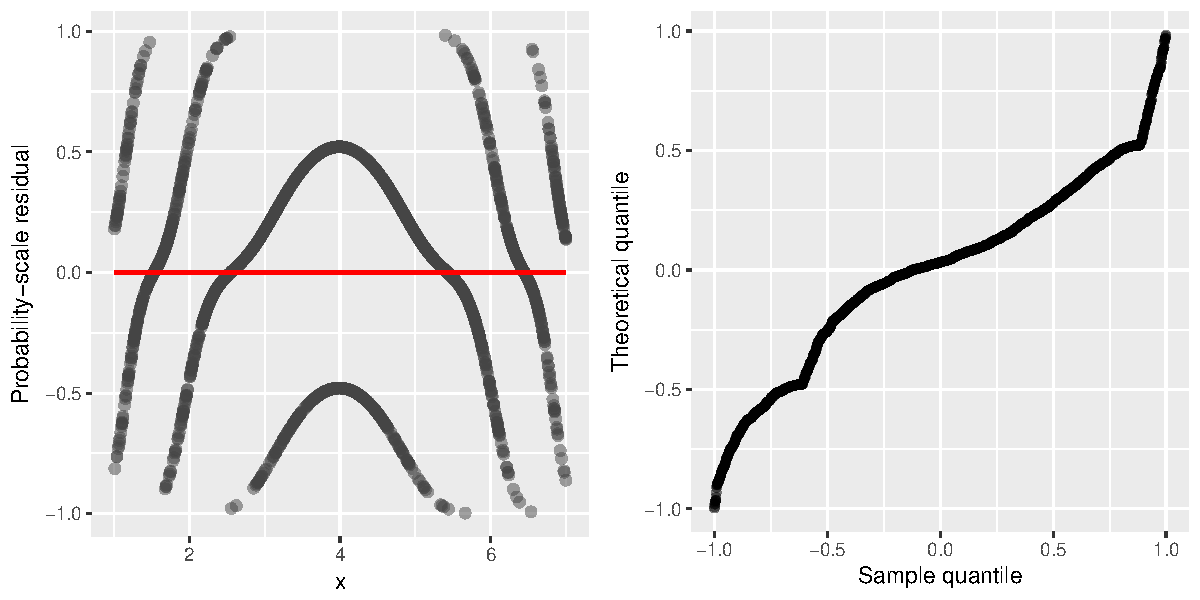
\includegraphics[width=1\textwidth]{quadratic-correct-sbs}
  \caption{SBS residual plots for the (correctly specified) probit model fit to the \code{df1} data set. \textit{Left}: Residual vs. covariate plot. \textit{Right}: Q-Q plot of the residuals. Nonparametric smooths are indicated by red curves.}
  \label{fig:quadratic-correct-sbs}
\end{figure}

Similarly, we can use the \code{resids} function in package \pkg{sure} to obtain the surrogate-based residuals discussed in Section~\ref{sec:surrogate}. This is illusratted in the following code chunk. the results are displayed in Figure~\ref{fig:quadratic-correct-surrogate}.
\begin{example}
# Load required package(s)
library(ggplot2)
library(sure)

# Obtain surrogate-based residuals
set.seed(101)  # for reproducibility
sres <- resids(fit.polr)

# Residual vs. covariate plot
p1 <- autoplot(sres, what = "covariate", x = df1$x, xlab = "x")

# Q-Q plot of the residuals
p2 <- autoplot(sres, what = "qq", distirbution = pnorm)

# Figure ?
grid.arrange(p1, p2, ncol = 2)
\end{example}
\begin{figure}[!htbp]
  \centering
  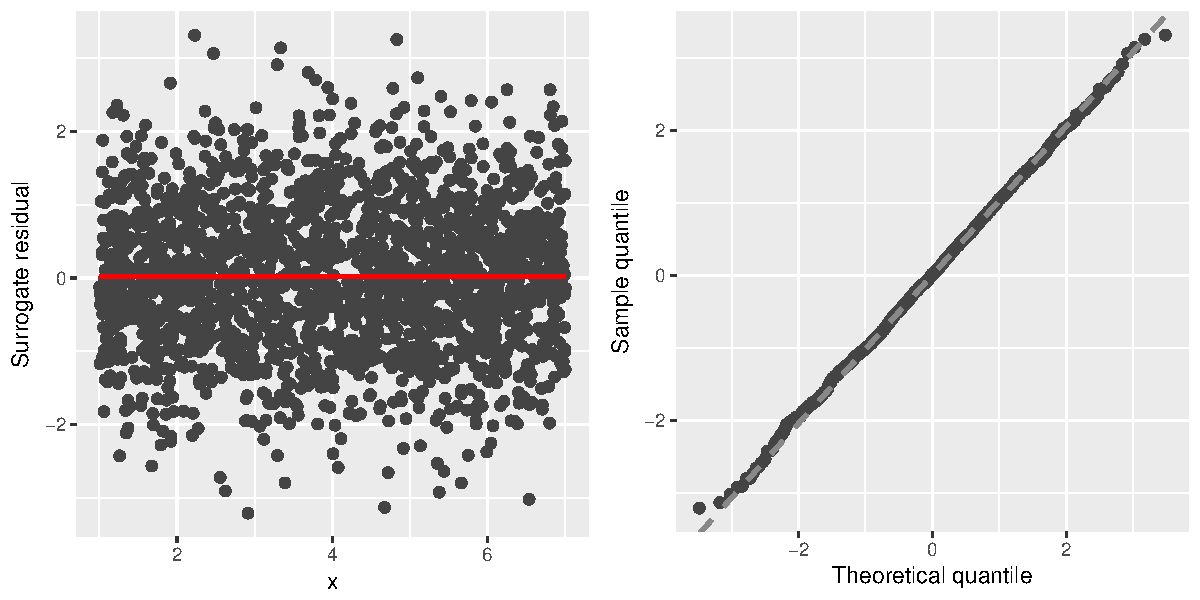
\includegraphics[width=1\textwidth]{quadratic-correct-surrogate}
  \caption{Surrogate-based residual plots for the (correctly specified) probit model fit to the \code{df1} data set. \textit{Left}: Residual vs. covariate plot. \textit{Right}: Q-Q plot of the residuals. Nonparametric smooths are indicated by red curves.}
  \label{fig:quadratic-correct-surrogate}
\end{figure}

We also wrote \code{autoplot} methods for various classes of models listed in Table~\ref{tab:pkgs}, so you can just give \code{autoplot} the fitted model directly. The benefit of this approach is that the fitted values and reference distirbution (used in quantile-quantile plots) are automatically extracted. For example, to reproduce the Q-Q plot in Figure~\ref{fig:quadratic-correct-surrogate}, we could have just used
\begin{example}
set.seed(101)  # for reproducibility
autoplot(fit.polr, what = "qq")  # same as top right of Figure 1
\end{example}

Suppose that we did not include the quadratic term in our fitted model. We could expect a residual-vs-$x$ plot to clearly indicate that such a (correct) quadratic term is missing. Below we update the previously fitted model by removing the quadratic term, then update the residual-vs-covariate plots (code not shown). The updated residual plots are displayed in Figure~\ref{fig:quadratic}.
\begin{example}
fit.polr <- update(fit.polr, y ~ x)  # remove quadratic term
\end{example}
The SBS residuals gives some indication of a misspecified mean structure, but this only becomes more clear with increasing $J$, and the plot is still discrete. This is overcome by the surrogate residuals which produces a residual plot not unlike those seen in ordinary linear regresion models.

\begin{figure}[!htbp]
  \centering
  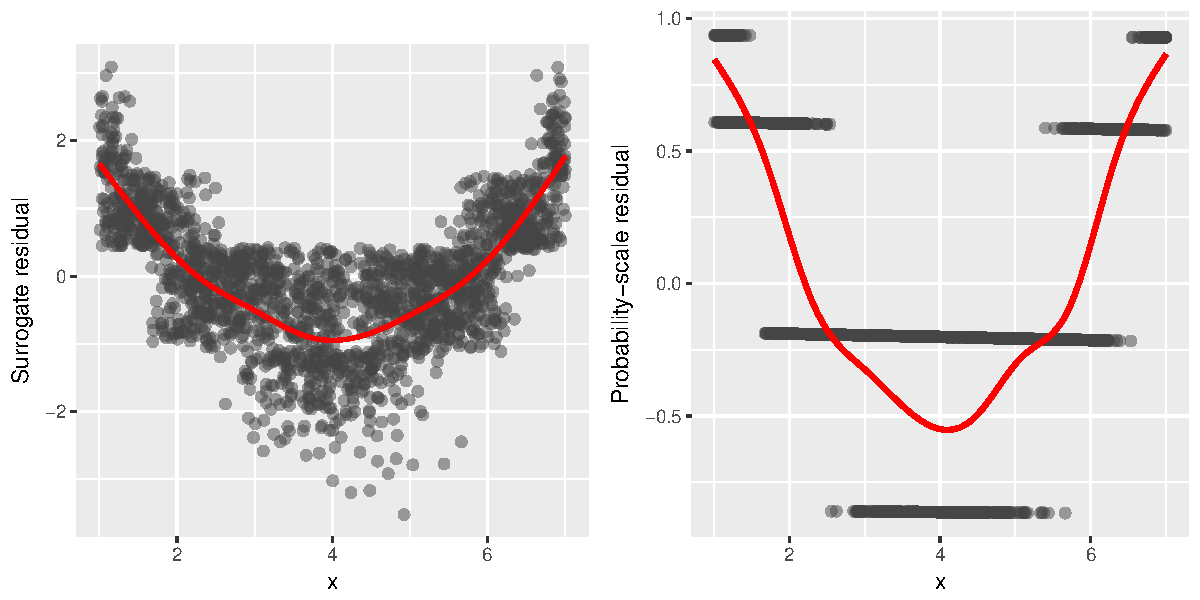
\includegraphics[width=1\textwidth]{quadratic}
  \caption{Residual-vs-covariate plots for a probit model with a misspecified mean structure fit to the simulated data from model \eqref{eqn:quadratic}. \textit{Left}: Surrogate residuals. \textit{Right}: SBS residuals. Nonparametric smooths are indicated by red curves.}
  \label{fig:quadratic}
\end{figure}


%%%%%%%%%%%%%%%%%%%%%%%%%%%%%%%%%%%%%%%%%%%%%%%%%%%%%%%%%%%%%%%%%%%%%%%%%%%%%%%%
\subsection{Detecting heteroscedasticty}
%%%%%%%%%%%%%%%%%%%%%%%%%%%%%%%%%%%%%%%%%%%%%%%%%%%%%%%%%%%%%%%%%%%%%%%%%%%%%%%%

One issue that oftens raises concerns in  stataistical inference is that of heteroscedasticity; that is, when the error term has non constant variance. Heteroscedasticity can bias the statistical infeence and lead to improper standard errors, confidence intervals, and $p$-values. Therefore, it is imperative to identify heteroscedacticity whenever present and take appropriate action (e.g., transformations, etc.). In ordinary linear regression, this topic has been covered extensively. For categorical models, on the other hand, not much has been proposed in the literature.

As discussed in Section~\ref{sec:surrogate}, one of the properties of the surrogate-based residual $R_\mathcal{S}$ is that, if the model is specified correctly, then $Var\left(R_\mathcal{S} | X\right) = c$, where $c$ is a contant.

For this example, we generated $n = 2000$ observations from the following ordered probit model:
\begin{equation*}
  Pr\left\{\mathcal{Y} \le j\right\} = \Phi\left\{\left(\alpha_j + \beta X\right) / \sigma_X\right\}, \quad j = 1, 2, 3, 4, 5,
\end{equation*}
where $\alpha_1 = -36$, $\alpha_2 = -6$, $\alpha_3 = 34$, $\alpha_4 = 64$, $\beta = -4$, $X \sim \mathcal{U}\left(2, 7\right)$, and $\sigma_X = X ^ 2$.
Notice how the variability is an increasing function of $X$. These data are available in the \code{df2} data frame that is automatically loaded with the \pkg{sure} package; see \code{?df2} for details.

The following block of code uses the \code{orm} function from the popular \pkg{rms} package to fit a probit model to the simulated data. \strong{Note} that we had to set \code{x = TRUE} in the call to \code{orm} in order to use the \code{presid} function later.
\begin{example}
# Load required package(s)
library(rms)

# Fit a cumulative link model with probit link
fit.orm <- orm(y ~ x, data = df2, family = "probit", x = TRUE)
\end{example}

If heteroscedasticity is present, we would expect this to show up in various diagnostic plots, such as a residual vs. covariate plot in this case. Below we obtain the SBS and surrogate residuals as before and plot them against $X$. The results are displayed in Figure~\ref{fig:heteroscedasticity}.
\begin{example}
pres <- presid(fit.orm)  # SBS residuals
set.seed(102)  # for reproducibility
sres <- resids(fit.orm)  # surrogate residuals

# Residual vs. covariate plots
p1 <- autoplot(sres, what = "covariate", x = df2$x, xlab = "x")
p2 <- ggplot(data.frame(x = df2$x, y = presid(fit.orm)), aes(x, y)) +
  geom_point(size = 2, alpha = 0.25) +
  geom_smooth(col = "red", se = FALSE) +
  ylab("Probability scale residual")
  
# Figure ?
grid.arrange(p1, p2, ncol = 2)
\end{example}

In Figure~\ref{fig:heteroscedasticity}, it is clear from the plot of the surrogate residuals (left side of Figure~\ref{fig:heteroscedasticity}) that the variance increases with $X$, a clear sign of heteroscedasticity. As a matter fact, the plot suggests that the true link function has a varying scale parameter, $\sigma = \sigma\left(\boldsymbol{X}\right)$. The plot of the SBS residuals (right side of Figure~\ref{fig:heteroscedasticity}), on the other hand, gives no indication of an issue with nonconstant variance.

\begin{figure}[!htbp]
  \centering
  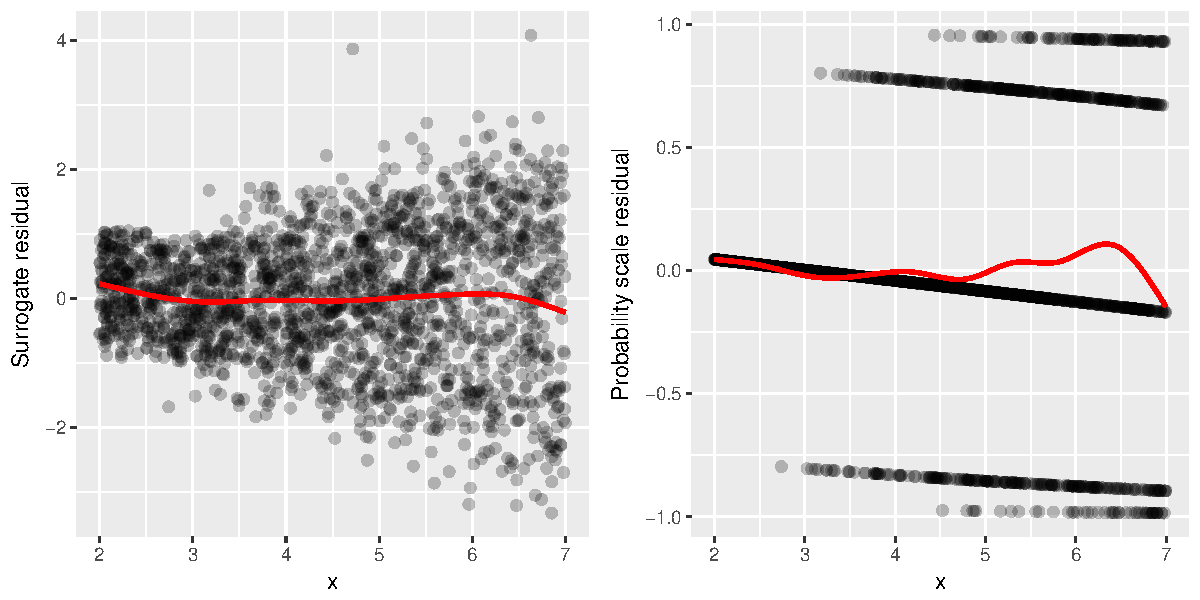
\includegraphics[width=1\textwidth]{heteroscedasticity}
  \caption{Residual vs. covariate plots for the simulated data. \textit{Left}: Surrogate residuals. \textit{Right}: SBS residuals.}
  \label{fig:heteroscedasticity}
\end{figure}


% %%%%%%%%%%%%%%%%%%%%%%%%%%%%%%%%%%%%%%%%%%%%%%%%%%%%%%%%%%%%%%%%%%%%%%%%%%%%%%%%
% \subsection{Detecting a misspecified link function}
% %%%%%%%%%%%%%%%%%%%%%%%%%%%%%%%%%%%%%%%%%%%%%%%%%%%%%%%%%%%%%%%%%%%%%%%%%%%%%%%%
% 
% For this example, we simulated $n = 2000$ observations from the quadratic model, but using a $\log$-$\log$ link.
% 
% \begin{example}
% data(df3, package = "sure")
% fit.probit <- polr(y ~ x + I(x ^ 2), data = df3, method = "probit")
% fit.logistic <- polr(y ~ x + I(x ^ 2), data = df3, method = "logistic")
% fit.loglog <- polr(y ~ x + I(x ^ 2), data = df3, method = "loglog")  # correct link
% fit.cloglog <- polr(y ~ x + I(x ^ 2), data = df3, method = "cloglog")
% \end{example}
% 
% \begin{example}
% # Figure ?
% p1 <- autoplot(fit.probit, nsim = 100, what = "qq")
% p2 <- autoplot(fit.logistic, nsim = 100, what = "qq")
% p3 <- autoplot(fit.loglog, nsim = 100, what = "qq")
% p4 <-  autoplot(fit.cloglog, nsim = 100, what = "qq")
% grid.arrange(p1, p2, p3, p4, ncol = 2)  # bottom left plot is correct model
% \end{example}
% 
% 
% %%%%%%%%%%%%%%%%%%%%%%%%%%%%%%%%%%%%%%%%%%%%%%%%%%%%%%%%%%%%%%%%%%%%%%%%%%%%%%%%
% \subsection{Checking the proportionality assumption}
% %%%%%%%%%%%%%%%%%%%%%%%%%%%%%%%%%%%%%%%%%%%%%%%%%%%%%%%%%%%%%%%%%%%%%%%%%%%%%%%%
% 
% Coming soon!
% 
% 
% %%%%%%%%%%%%%%%%%%%%%%%%%%%%%%%%%%%%%%%%%%%%%%%%%%%%%%%%%%%%%%%%%%%%%%%%%%%%%%%%
% \subsection{Assessing goodness-of-fit}
% %%%%%%%%%%%%%%%%%%%%%%%%%%%%%%%%%%%%%%%%%%%%%%%%%%%%%%%%%%%%%%%%%%%%%%%%%%%%%%%%
% 
% Coming soon!
% 
% \begin{example}
% plot(gof(houses.polr, nsim = 1000))
% \end{example}
% 
% 
% %%%%%%%%%%%%%%%%%%%%%%%%%%%%%%%%%%%%%%%%%%%%%%%%%%%%%%%%%%%%%%%%%%%%%%%%%%%%%%%%
% \section{Bitterness of wine}
% %%%%%%%%%%%%%%%%%%%%%%%%%%%%%%%%%%%%%%%%%%%%%%%%%%%%%%%%%%%%%%%%%%%%%%%%%%%%%%%%
% 
% \begin{example}
% library(ordinal)
% data(wine, package = "ordinal")
% wine.clm <- clm(rating ~ temp * contact, data = wine)  # default logit link
% \end{example}
% 
% \begin{example}
% set.seed(101)  # for reproducibility
% grid.arrange(
%   autoplot(wine.clm, nsim = 10, what = "qq"),
%   autoplot(wine.clm, nsim = 10, what = "fitted"),
%   autoplot(wine.clm, nsim = 10, what = "cov", x = wine$temp),
%   autoplot(wine.clm, nsim = 10, what = "cov", x = wine$contact),
%   ncol = 2
% )
% \end{example}
% 
% \begin{figure}[!htbp]
%   \centering
%   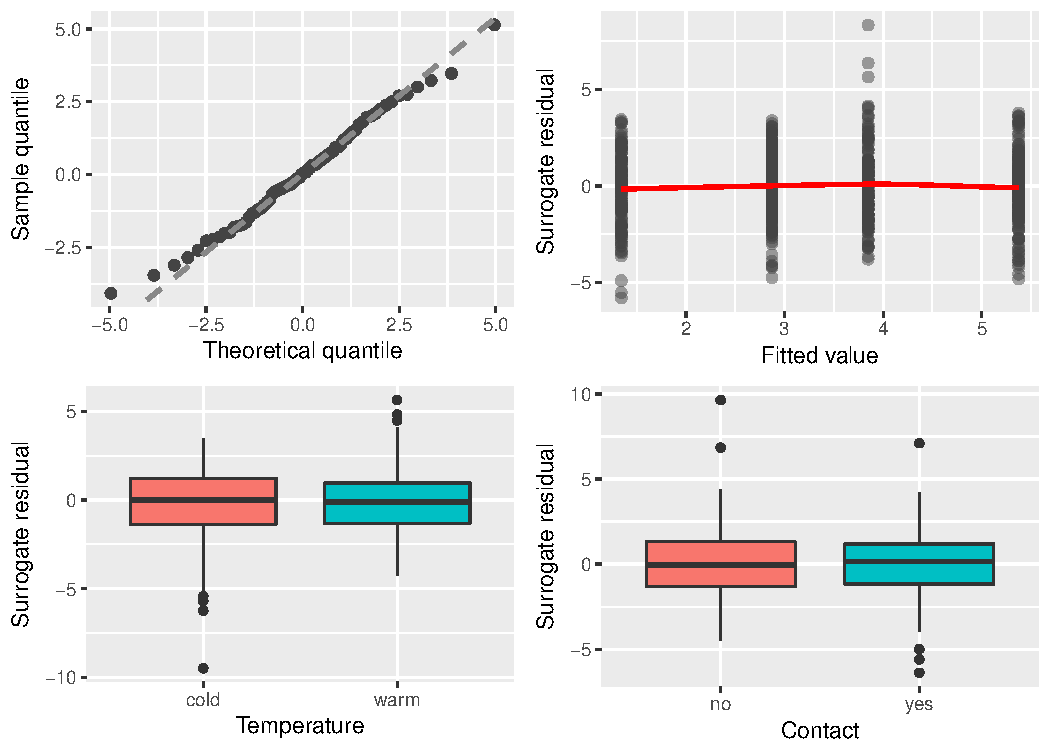
\includegraphics[width=1\textwidth]{wine}
%   \caption{Residual diagnostic plots for the quality of wine example.}
%   \label{fig:wine}
% \end{figure}
% 


%%%%%%%%%%%%%%%%%%%%%%%%%%%%%%%%%%%%%%%%%%%%%%%%%%%%%%%%%%%%%%%%%%%%%%%%%%%%%%%%
\section{Summary}
%%%%%%%%%%%%%%%%%%%%%%%%%%%%%%%%%%%%%%%%%%%%%%%%%%%%%%%%%%%%%%%%%%%%%%%%%%%%%%%%

TBD.


%%%%%%%%%%%%%%%%%%%%%%%%%%%%%%%%%%%%%%%%%%%%%%%%%%%%%%%%%%%%%%%%%%%%%%%%%%%%%%%%
\section{Acknowledgments}
%%%%%%%%%%%%%%%%%%%%%%%%%%%%%%%%%%%%%%%%%%%%%%%%%%%%%%%%%%%%%%%%%%%%%%%%%%%%%%%%

TBD.


\bibliography{greenwell-lastname2-lastname3}

\address{Author One\\
  Affiliation\\
  Address\\
  Country\\
  (ORCiD if desired)\\
  \email{author1@work}}

\address{Author Two\\
  Affiliation\\
  Address\\
  Country\\
  (ORCiD if desired)\\
  \email{author2@work}}

\address{Author Three\\
  Affiliation\\
  Address\\
  Country\\
  (ORCiD if desired)\\
  \email{author3@work}}
